\documentclass[letterpaper,9pt,twocolumn,twoside,]{pinp}

%% Some pieces required from the pandoc template
\providecommand{\tightlist}{%
  \setlength{\itemsep}{0pt}\setlength{\parskip}{0pt}}

% Use the lineno option to display guide line numbers if required.
% Note that the use of elements such as single-column equations
% may affect the guide line number alignment.

\usepackage[T1]{fontenc}
\usepackage[utf8]{inputenc}

% pinp change: the geometry package layout settings need to be set here, not in pinp.cls
\geometry{layoutsize={0.95588\paperwidth,0.98864\paperheight},%
  layouthoffset=0.02206\paperwidth, layoutvoffset=0.00568\paperheight}

\definecolor{pinpblue}{HTML}{185FAF}  % imagecolorpicker on blue for new R logo
\definecolor{pnasbluetext}{RGB}{0,101,165} % default in pinp.cls


\usepackage{float}

\title{Predicting House Prices in New York Using Multiple Regression
Analysis}

\author[]{Abtahee Islam}


\setcounter{secnumdepth}{5}

% Please give the surname of the lead author for the running footer
\leadauthor{}

% Keywords are not mandatory, but authors are strongly encouraged to provide them. If provided, please include two to five keywords, separated by the pipe symbol, e.g:
 \keywords{  Housing Prices |  Multiple Linear Regression |  Property
features |  Neighbourhood features  }  

\begin{abstract}
We analyse 1,734 New York housing sales to identify which property and
neighbourhood features best predict sale prices. Predictors include
living area, land value, age, bathrooms, and neighbourhood indicators
such as the share of college-educated residents and waterfront access.
After data cleaning and stepwise variable selection, we compared a
multiple linear regression with a random forest model. Living area and
land value were dominant predictors. The final seven-predictor linear
model explained about 63.7\% of price variation while the random forest
captured diminishing returns and mild non-linearities. Overall, property
size and land worth mainly drive most pricing differences, while
neighbourhood quality has smaller effects.
\end{abstract}

\dates{This version was compiled on \today} 


% initially we use doi so keep for backwards compatibility
% new name is doi_footer
\doifooter{\url{https://github.com/FromScratchToDataScientist/House-Price-Prediction-NYC-}}

\pinpfootercontents{House Prices Analysis Vignette}

\begin{document}

% Optional adjustment to line up main text (after abstract) of first page with line numbers, when using both lineno and twocolumn options.
% You should only change this length when you've finalised the article contents.
\verticaladjustment{-2pt}

\maketitle
\thispagestyle{firststyle}
\ifthenelse{\boolean{shortarticle}}{\ifthenelse{\boolean{singlecolumn}}{\abscontentformatted}{\abscontent}}{}

% If your first paragraph (i.e. with the \dropcap) contains a list environment (quote, quotation, theorem, definition, enumerate, itemize...), the line after the list may have some extra indentation. If this is the case, add \parshape=0 to the end of the list environment.

\acknow{This template package builds upon, and extends, the work of the
excellent \href{https://cran.r-project.org/package=rticles}{rticles}
package, and both packages rely on the
\href{http://www.pnas.org/site/authors/latex.xhtml}{PNAS LaTeX} macros.
Both these sources are gratefully acknowledged as this work would not
have been possible without them. Our extensions are under the same
respective licensing term
(\href{https://www.gnu.org/licenses/gpl-3.0.en.html}{GPL-3} and
\href{https://www.latex-project.org/lppl/}{LPPL (\textgreater= 1.3)}).}

\subsection{Introduction}\label{introduction}

Understanding what drives house prices is important for buyers and
developers in New York. The diverse housing market, with large variation
in property types and neighborhood amenities, offers interesting
insight. Our study asks: Which property and neighborhood factors best
predict New York house prices, and how do model choices affect this? We
examine multiple variables describing structural and socioeconomic
features of each property. After exploratory analysis and processing, we
fit and compare two predictive models: a transparent multiple linear
regression for interpreting variable effects, and a random forest to
capture potential non-linear relationships. The sections that follow
outline the data and cleaning process, model specification and
diagnostics, key results, and practical implications.

\subsection{Dataset}\label{dataset}

The dataset used in this study is a random sample of 1,734 residential
properties drawn from the full Saratoga Housing Data (De Veaux, 2019),
containing information on residential properties sold in Saratoga
County, New York. Each observation includes 17 variables describing key
property features and neighborhood characteristics. Key variables
include:

\begin{itemize}
\tightlist
\item
  \textbf{Price}: sale price of the property in USD
\item
  \textbf{Living.Area}: interior living area in square feet
\item
  \textbf{Pct.College}: proportion of neighborhood residents with a
  college degree
\item
  \textbf{Bedrooms}: number of bedrooms
\item
  \textbf{Bathrooms}: number of bathrooms
\item
  \textbf{Land.Value}: assessed land value in USD
\item
  \textbf{Age}: property age in years
\item
  \textbf{Lot.Size}: total land area in square feet
\end{itemize}

\subsection{Analysis}\label{analysis}

The aim of this analysis was to identify property and neighborhood
features that best predict housing prices in New York. A structured
multiple regression approach involving exploratory data analysis,
systematic model selection, and assumption checking was used to identify
the most influential predictors and evaluate how well they explain the
variations in house prices. The analysis started with data cleaning and
transformation. First, the data was cleaned to remove any missing or
invalid entries. Key categorical variables (Waterfront, Central.Air and
New.Construct) were converted into factors for appropriate treatment in
regression modelling. Exploratory data analysis was performed to explore
relationships between variables. The correlation heatmap (Appendix,
Fig.1.) revealed strong positive correlations between Price and both
Living.Area and Land.Value, moderate correlations with Bathrooms and
Pct.College and a negative relationship with Age. These insights
provided initial guidance on variables likely to influence house prices
and informed subsequent regression modelling decisions.

Stepwise regression using the Akaike Information Criterion (AIC) was
performed in both forward and backward directions to select a
parsimonious and well-fitting model. Forward selection started with an
empty model with only the intercept and sequentially added predictors
that most improved AIC. Forward stepwise regression selected a model
containing the variables Living.Area, Land.Value, Bathrooms, Waterfront,
Age, Rooms and Fireplaces (Appendix Fig.2.). On the other hand, backward
elimination started with a full model and iteratively eliminated
variables if removing them improved AIC. Backward selection converged to
an identical model with the same seven predictor variables (Appendix
Fig.2.) indicating strong model stability.

To further validate the stepwise regression results and explore all
possible variable combinations, an exhaustive subset selection was
performed using the Bayesian Information Criterion (BIC). The best BIC
model included the variables Living.Area, Land.Value, Bathrooms,
Waterfront, Age and Pct.College (Appendix, Fig.3.). There are two
notable differences between this model and the stepwise AIC model.
Unlike the stepwise AIC models, the BIC model includes the variable
Pct.College but excludes Rooms and Fireplaces. The exhaustive search
heatmap (Appendix, Fig.3.) reveals that all the top-performing models
consistently included Living.Area, Land.Value, Age, Bathrooms, and
Waterfront. This highlights the strong influence of these variables as
predictors of house prices.

After comparing the models, the stepwise AIC model including seven
predictor variables was chosen as the final regression model due to
various reasons. Firstly, both the forwards selection and backwards
elimination method converged to this model, displaying great model
stability. Moreover, cross-validation results also confirmed excellent
model generalisability with minimal overfitting. Overall, this model
also maintained excellent interpretability, including predictors
representing both property features as well as neighborhood
characteristics.

Ten-fold cross-validation was performed to evaluate model performance
and generalisability. The dataset was partitioned into ten equal subsets
(folds), with nine folds used for training and one fold used for
testing. The cross-validation results (Appendix, Fig.5.) showed that the
model achieved:RMSE value of 59,540.07 (root mean squared error),
\(R^2\) of 0.641 (cross-validated coefficient of determination) and MAE
of 42,304.71 (mean absolute error).

The cross-validated \(R^2\)(0.641) was very close to the training
\(R^2\)(0.637), which indicates strong predictive performance, good
generalisability to unseen data and minimal overfitting.

The final multiple linear regression model took the form: \[
\begin{aligned}
\text{Price} = & \ 9948.18 + 65.36 \, (\text{Living.Area}) + 0.92 \, (\text{Land.Value}) \\
               & + 22508.57 \, (\text{Bathrooms}) + 125860.16 \, (\text{Waterfront}) \\
               & - 182.08 \, (\text{Age}) + 1975.48 \, (\text{Rooms}) + 4469.08 \, (\text{Fireplaces}) \\
               & + \epsilon
\end{aligned}
\]

The model explained approximately 63.7\% of the variance in Price
(\(R^2 = 0.637\), \(R^2_{\text{Adj.}} = 0.635\)). The coefficients can
be interpreted as follows:

\begin{itemize}
\tightlist
\item
  \textbf{Living.Area} (\(\beta = 65.36\), \(p < 0.01\)): Each
  additional square foot of living area increases Price by \$65.36.
\item
  \textbf{Land.Value} (\(\beta = 0.92\), \(p < 0.01\)): Each additional
  dollar of land value increases price by \$0.92.
\item
  \textbf{Bathrooms} (\(\beta = 22508.57\), \(p < 0.01\)): Each
  additional bathroom significantly increases Price by \$22,508.57.
\item
  \textbf{Waterfront} (\(\beta = 125860.16\), \(p < 0.01\)): Waterfront
  houses increase price by \$125,860.16.
\item
  \textbf{Age} (\(\beta = -182.08\), \(p < 0.01\)): Every additional
  year of property age decreases price by \$182.08.
\item
  \textbf{Rooms} (\(\beta = 1975.48\), \(p = 0.03\)): Every additional
  room increases Price by \$1,975.48.
\item
  \textbf{Fireplaces} (\(\beta = 4469.08\), \(p = 0.13\)): Each
  additional fireplace increases Price by \$4,469.08; however, this
  effect is not statistically significant at \(\alpha = 0.05\).
\end{itemize}

The final model was assessed for all key regression assumptions:

\begin{itemize}
\tightlist
\item
  \textbf{Linearity}: Residual vs.~Fitted plot (Appendix, Fig.6.)
  displayed points randomly scattered around zero, confirming
  appropriate linear specification between the selected predictors and
  house prices.
\item
  \textbf{Normality}: Q-Q plot (Appendix, Fig.6.) indicated that
  residuals followed an approximately normal distribution, with minor
  deviations in the upper tail suggesting limited influence of heavy
  outliers.
\item
  \textbf{Independence}: The dataset consists of a random sample of
  properties drawn from the full Saratoga Housing dataset, which
  supports the independent observations assumption.
\item
  \textbf{Homoscedasticity}: The Scale-Location plot showed consistent
  spread of residuals across the range of fitted values and confirmed
  that the assumption was satisfied.
\item
  \textbf{Multicollinearity}: All Variance Inflation Factors (VIF)
  (Appendix, Fig.7.) remained below 5, indicating no substantial
  multicollinearity among the predictor variables.
\end{itemize}

Our analysis also tested a Random Forest model to explore non-linear
relationships, particularly for Bathrooms. This revealed diminishing
returns in price for properties with more than three bathrooms. However,
the Random Forest model only explained 36.49\% of the price variance
which is significantly lower than the linear model (\(R^2\)=0.64). As a
result, the regression model was preferred over the Random Forest model
as it offered greater predictive performance and interpretability.

\subsection{Results}\label{results}

After cleaning and transforming the data, the final dataset contained
1734 New York house prices. A combination of stepwise regression,
multipole linear regression, random forest modelling, and
cross-validation was used to identify key price drivers.

A stepwise model selection process was conducted that used both forward
and backward AIC search. Both procedures highlighted similar models as
they selected Living Area, Land Value, Age, Bathrooms, Waterfront,
Rooms, Fireplaces. The agreement between both directions suggest that
these predictors consistently provide the strongest fitted model. This
indicates that the selected features are strong contributors to
predicting housing prices, rather than appearing due to randomness or
noise.

Using the selected predictors, a multiple linear regression model was
fitted. The model explained approximately 63.7 \% of variance(\(R^2\) =
0.637) in housing prices, which indicates a strong predictive power for
a housing dataset with many different property types. The effects of
these predictors show that:

\begin{itemize}
\tightlist
\item
  Houses with larger living areas and higher land value sold for more.
\item
  Properties with waterfronts carry the largest price premium.
\item
  Older homes sell for less, reflecting how in the real-world house
  prices depreciate over time.
\item
  Additional bathrooms and rooms increased value bur diminish returns
  were noticeable.
\item
  Fireplaces had a small effect on price after other variables were
  accounted for.
\end{itemize}

Taken together, these estimates indicate that the final model captures
the major structural predictors of housing prices with strong
explanatory power.

A Random Forest model was used to explore potential non-linear
relations. With this model we captured diminishing returns in bathroom
count. Prices increase significantly from 1.5 -- 2.5 bathrooms but
slowed down when testing more than 3 bathrooms. This model explained
37\% of variance(\(R^2\) = 0.37) in housing prices. This shows that the
random forest was less interpretable, making it difficult to understand
of individual predictors on price.

A 10-fold cross-validated linear regression was used to test how well
the model works with other datasets. The cross-validation showed a
stable performance which indicates that the linear model is not
overfitting.

Overall, the results show that structural property features such as
living area, land value, bathrooms, and waterfront access are the most
important factors of affecting increase of housing prices. Neighbourhood
features had a weaker influence once structural features were included.
The final linear model provided the best accuracy and interpretability
which explained 63\% of variation in price.

\subsection{Discussion \& Conclusion}\label{discussion-conclusion}

The results collected show that living area and land value are the main
drivers of New York house prices. In the final multiple linear
regression model, both variables accounted for the most variation in
housing prices. Neighbourhood features, such as college-educated
residents or waterfront traits, add smaller price premiums if all
predictors are taken into account. The age predictor had a negative
effect on price reflecting depreciation of older houses. The random
forest model supported the same ranking of predictors and highlighted
some non-linear patterns. Ten-fold cross-validation showed stable
predictive accuracy suggesting that the linear model generalises well.
However, limitations are still present as the dataset does not include
key predictors such as renovation quality, sale dates or location. These
important influences will not be observed and price differences tied to
those predictors will be left unexplained, limiting the model's
predictive power. Including features like spatial data and time-based
information would likely improve predictive accuracy. Overall, property
size and land value explain most of price variation and the linear model
remains the most effective and interpretable for understanding how
individual predictors affect price.

\newpage

\section*{Appendix}\label{appendix}
\addcontentsline{toc}{section}{Appendix}

\begin{figure}[H]

{\centering 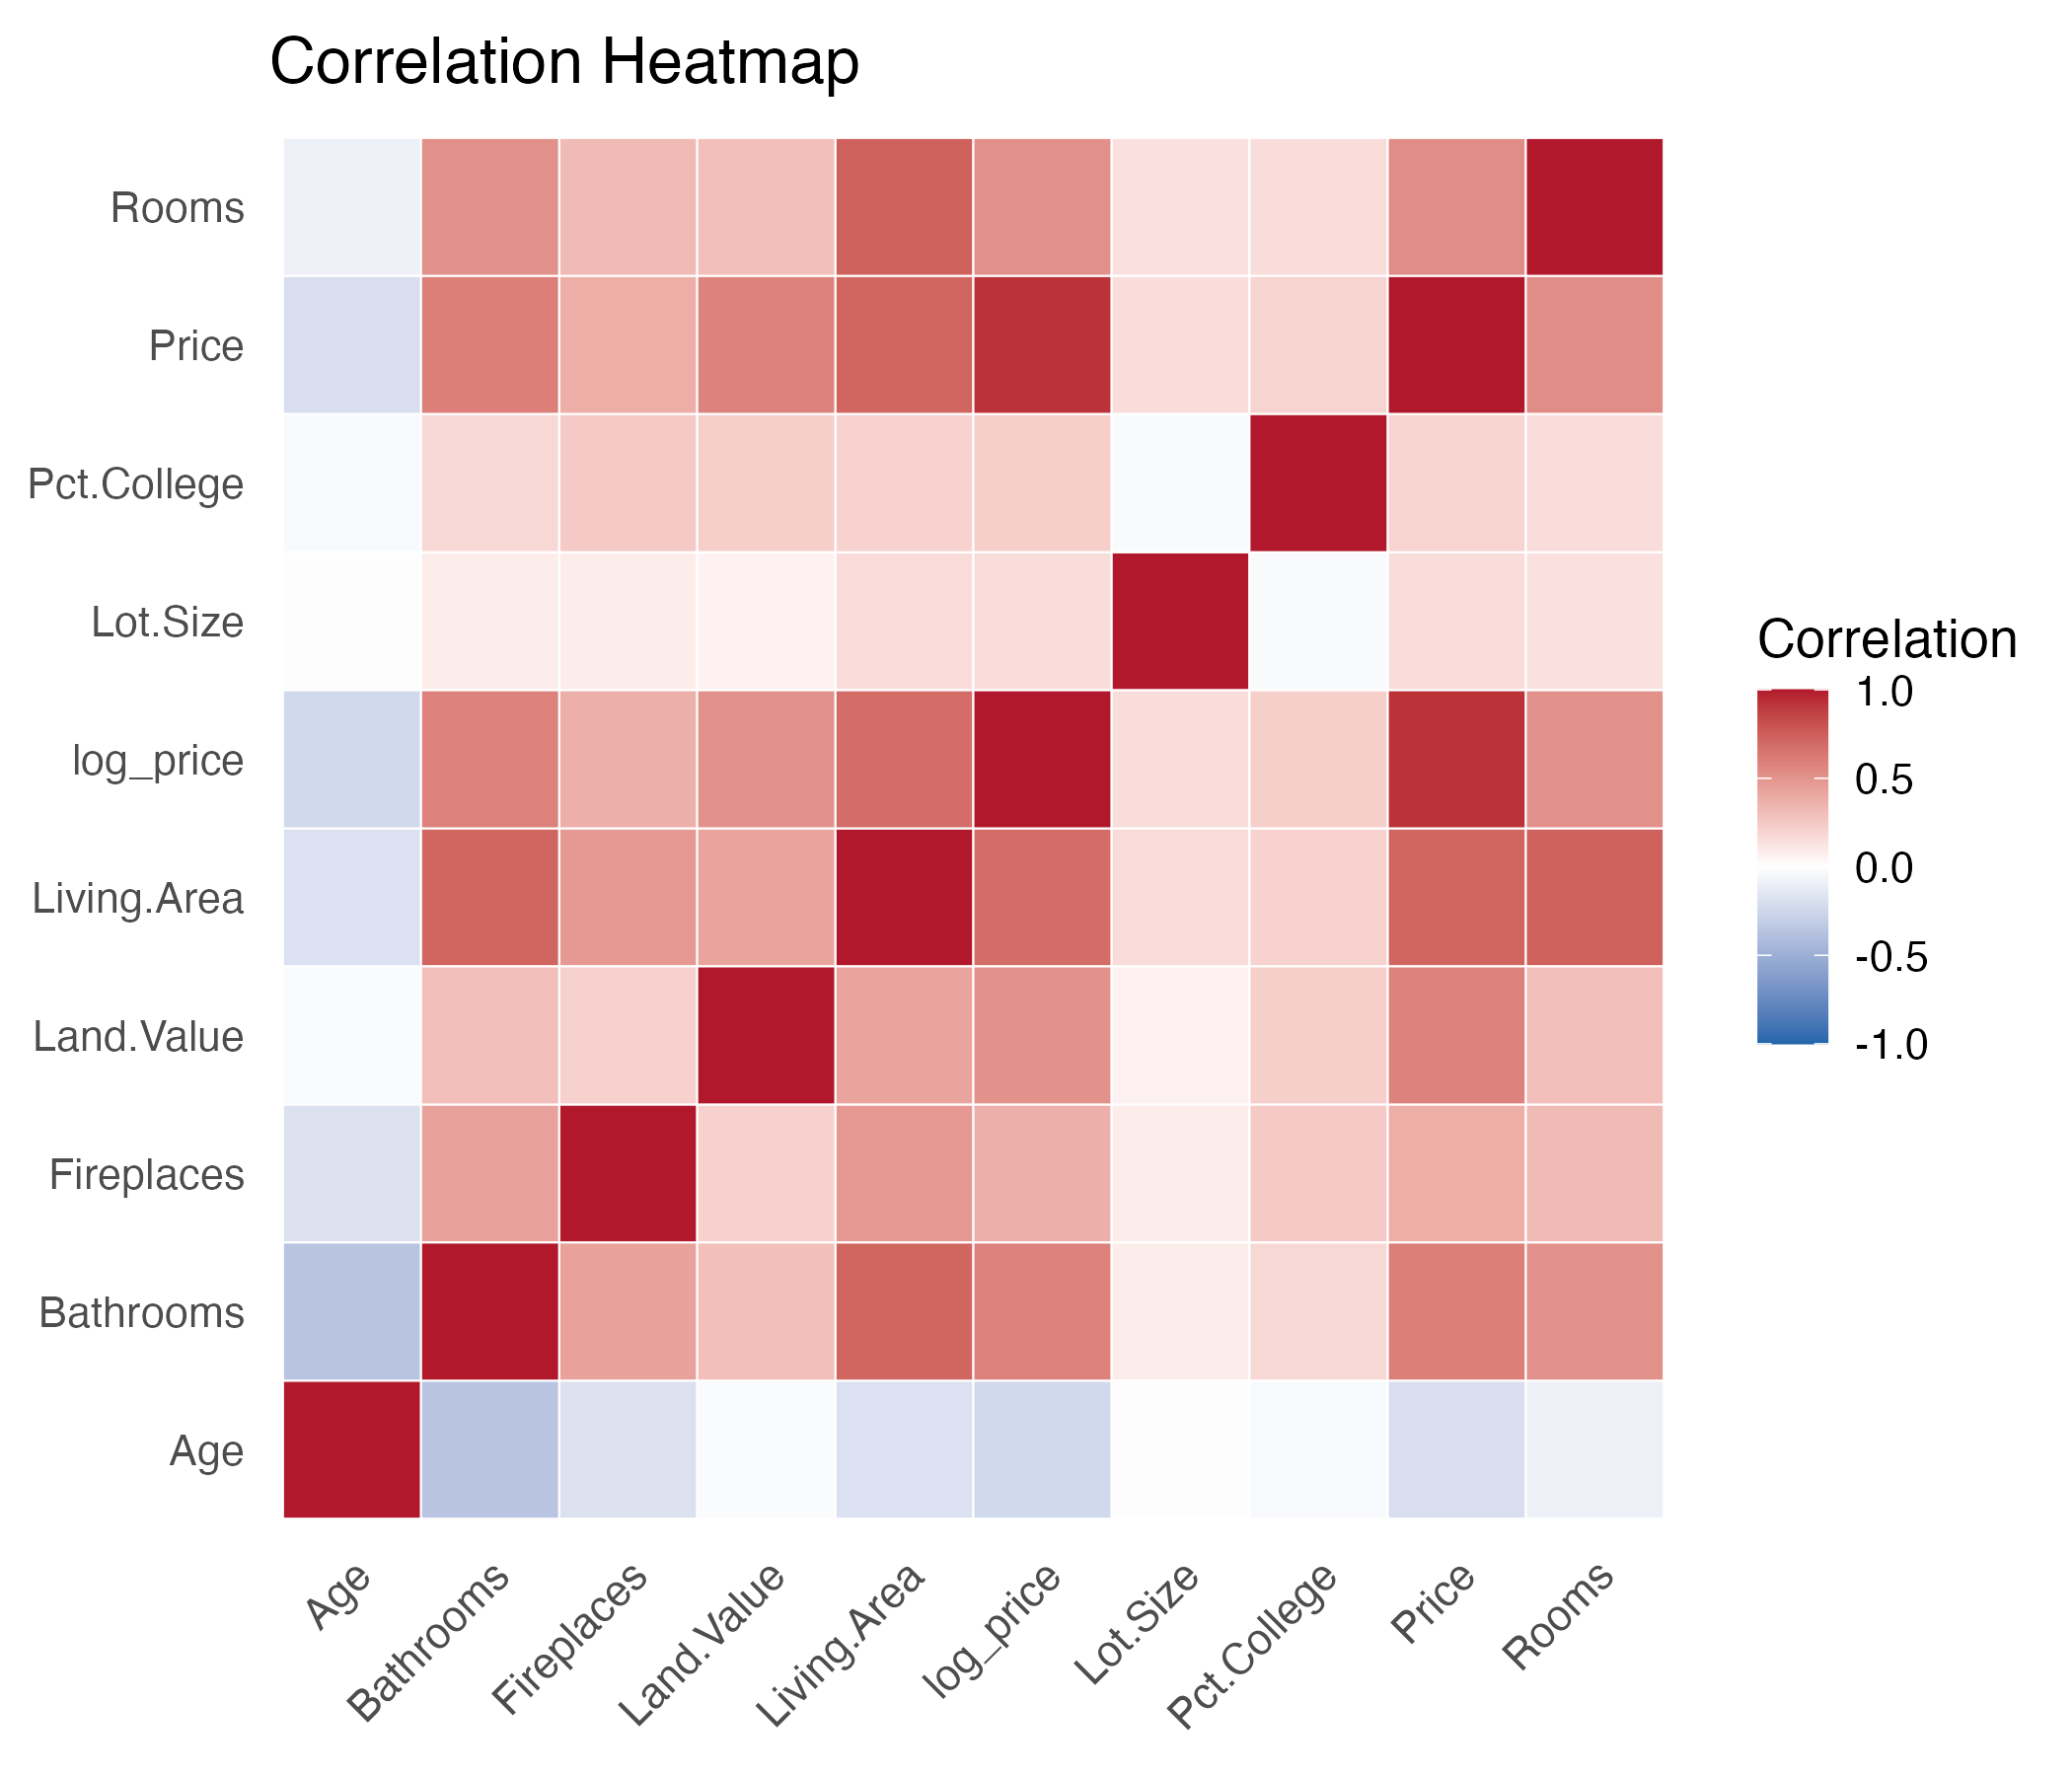
\includegraphics[width=0.7\linewidth]{correlation_heatmap} 

}

\caption{Correlation heatmap illustrating the relationships among key housing variables.}\label{fig:correlation_heatmap}
\end{figure}

\begin{figure}[H]

{\centering 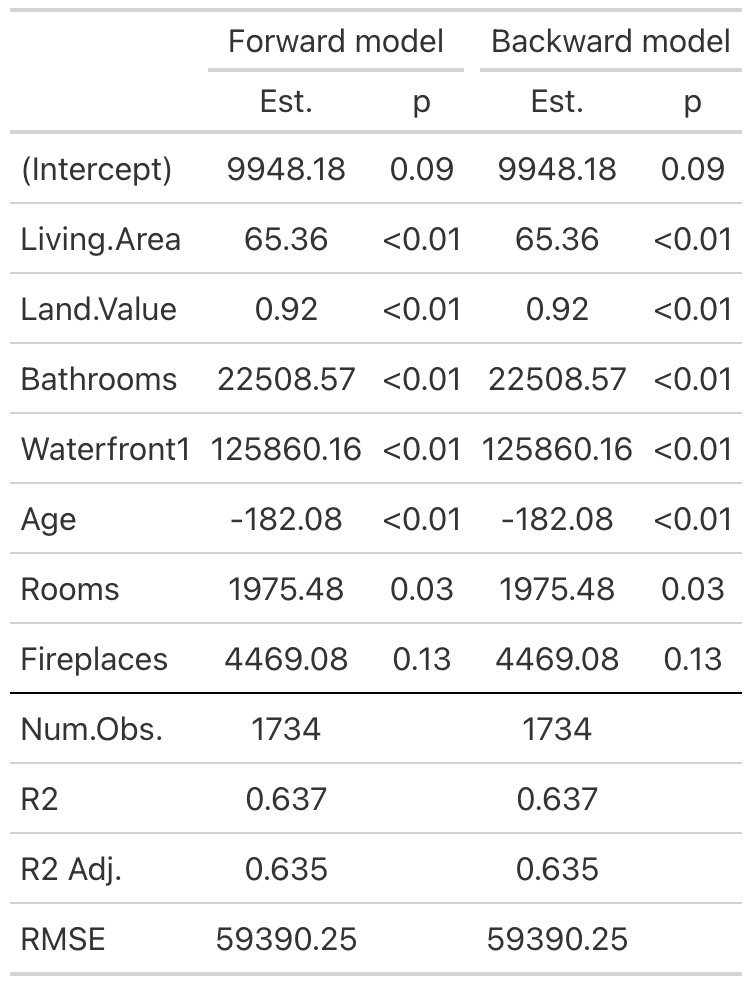
\includegraphics[width=0.5\linewidth]{stepwise_table} 

}

\caption{Stepwise regression table summarising variable entry and removal.}\label{fig:stepwise_table}
\end{figure}

\begin{figure}[H]

{\centering 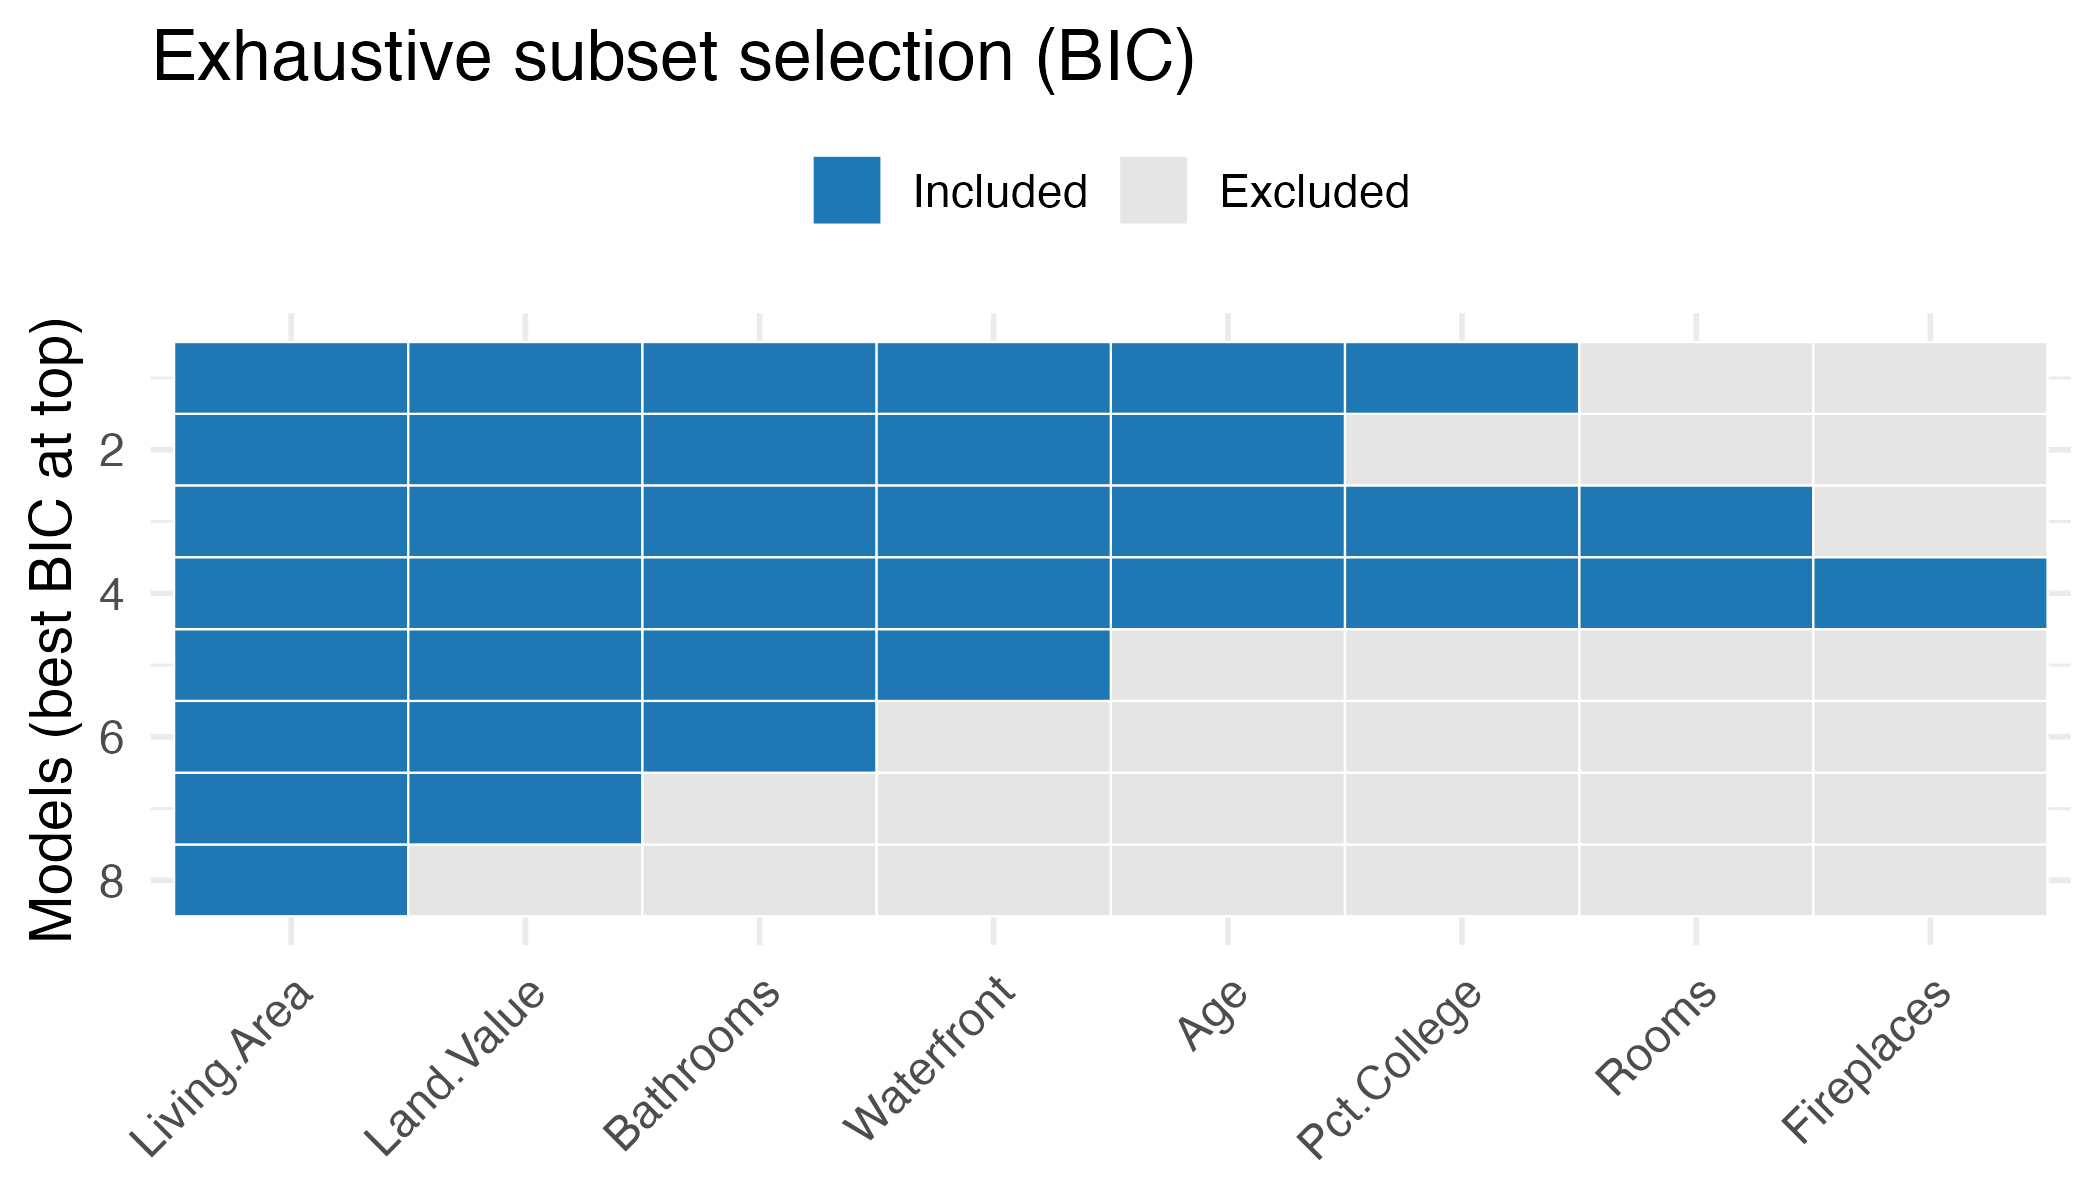
\includegraphics[width=0.7\linewidth]{exhaustive_heatmap} 

}

\caption{Exhaustive search heatmap showing model selection by criterion.}\label{fig:exhaustive_heatmap}
\end{figure}

\begin{figure}[H]

{\centering 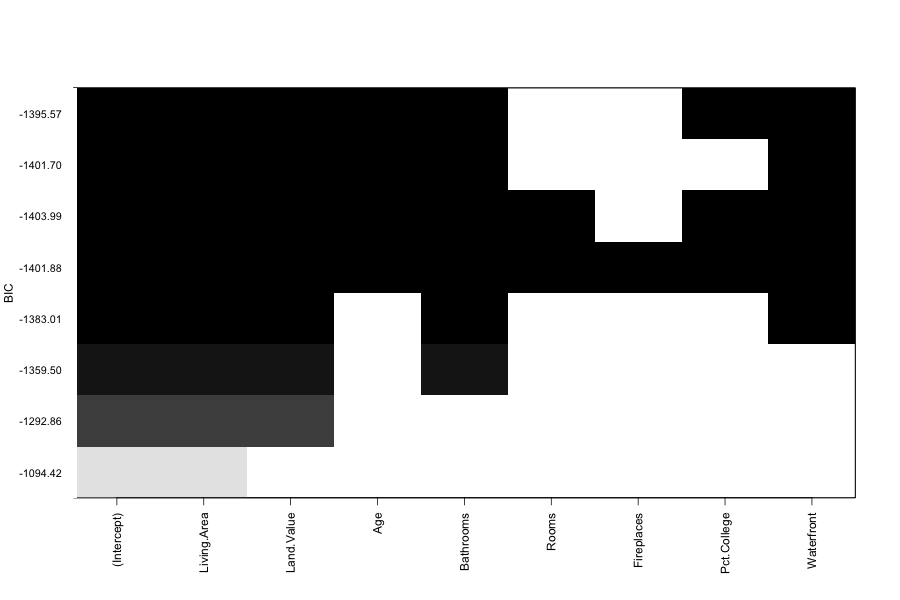
\includegraphics[width=0.7\linewidth]{regsubsets_BIC} 

}

\caption{Model selection using the Bayesian Information Criterion (BIC).}\label{fig:regsubsets_BIC}
\end{figure}

\begin{figure}[H]

{\centering 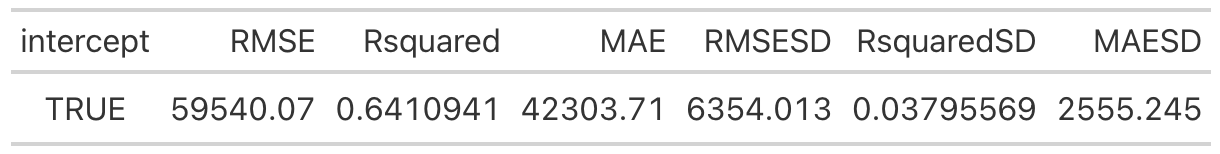
\includegraphics[width=0.7\linewidth]{cv_results} 

}

\caption{Cross-validation results comparing model performance across folds.}\label{fig:cv_results}
\end{figure}

\begin{figure}[H]

{\centering 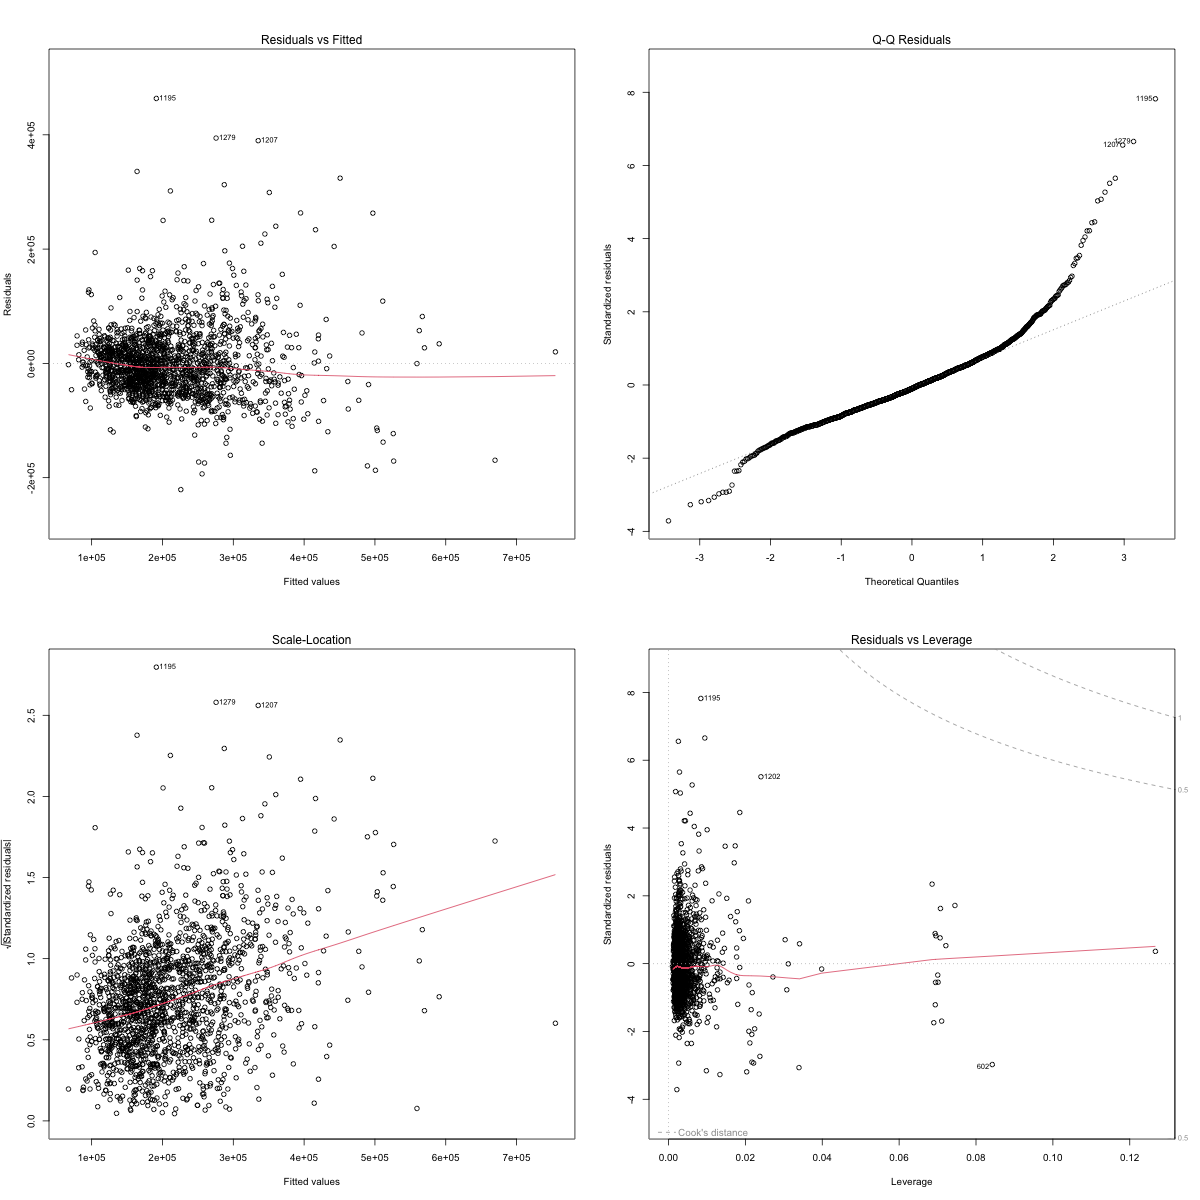
\includegraphics[width=0.7\linewidth]{diagnostics} 

}

\caption{Diagnostic plots for assessing regression assumptions}\label{fig:diagnostics}
\end{figure}

\begin{figure}[H]

{\centering 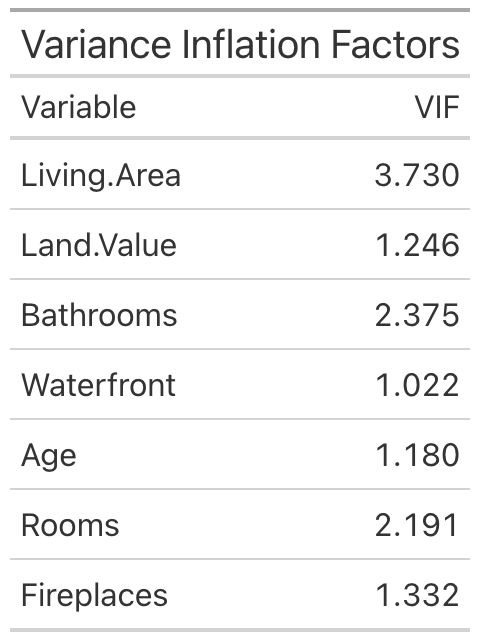
\includegraphics[width=0.4\linewidth]{vif} 

}

\caption{Variance Inflation Factors (VIF) for detecting multicollinearity.}\label{fig:vif}
\end{figure}

%\showmatmethods
\showacknow


\bibliography{pinp}
\bibliographystyle{jss}



\end{document}
